% =====================================================================
%  7. Résultats d'entraînement supervisé
% =====================================================================
\clearpage
\section{Résultats de l'entraînement supervisé}
\label{sec:resultats}

Cette section présente les résultats dans l'ordre où ils ont été obtenus : un
premier benchmark groupé avec la configuration initiale (13 entrées, imputation
itérative), puis les résultats de la configuration de travail (16 entrées,
imputation médiane) sous les deux scénarios de validation.

\subsection{Premier benchmark : 13 entrées, imputation itérative, validation groupée}
\label{subsec:bench13}

Le notebook 03 a exécuté les 100 évaluations externes (5 familles $\times$
4 cibles $\times$ 5 plis) en six minutes environ. Les 80 ajustements de
prétraitement ont convergé (3 à 20 itérations selon la cible et le pli). Le
\cref{tab:bench13} donne les scores.

\begin{table}[htbp]
\centering
\small
\caption{Premier benchmark, schéma 13/itérative, validation groupée : moyenne
$\pm$ écart-type sur les cinq plis externes. En gras : plus faible MAE par cible.}
\label{tab:bench13}
\begin{tabular}{@{}llrrr@{}}
\toprule
Cible & Modèle & MAE & RMSE & $R^2$ \\
\midrule
\multirow{5}{*}{\YS{} (MPa)}
 & Médiane de $y$ & 70,45 $\pm$ 10,68 & 92,50 & $-0{,}073$ \\
 & Ridge          & 69,92 $\pm$ 5,17  & 90,88 & $-0{,}054$ \\
 & SVR RBF        & 69,28 $\pm$ 12,81 & 89,26 & 0,004 \\
 & Forêt aléatoire & \meilleur{65,88 $\pm$ 10,61} & 85,65 & 0,079 \\
 & $k$NN          & 76,87 $\pm$ 15,75 & 98,68 & $-0{,}208$ \\
\midrule
\multirow{5}{*}{\UTS{} (MPa)}
 & Médiane de $y$ & 72,66 $\pm$ 15,24 & 93,73 & $-0{,}180$ \\
 & Ridge          & 65,88 $\pm$ 15,14 & 82,99 & 0,054 \\
 & SVR RBF        & 63,40 $\pm$ 12,70 & 83,43 & 0,039 \\
 & Forêt aléatoire & \meilleur{57,65 $\pm$ 10,78} & 76,25 & 0,194 \\
 & $k$NN          & 66,65 $\pm$ 16,00 & 88,66 & $-0{,}089$ \\
\midrule
\multirow{5}{*}{\makecell[l]{Allongement\\ (points de \%)}}
 & Médiane de $y$ & 4,09 $\pm$ 0,31 & 4,96 & $-0{,}062$ \\
 & Ridge          & 3,73 $\pm$ 0,31 & 4,57 & 0,094 \\
 & SVR RBF        & 3,88 $\pm$ 0,39 & 4,82 & $-0{,}007$ \\
 & Forêt aléatoire & \meilleur{3,56 $\pm$ 0,18} & 4,49 & 0,125 \\
 & $k$NN          & 3,91 $\pm$ 0,25 & 5,02 & $-0{,}093$ \\
\midrule
\multirow{5}{*}{\charpy{} (J)}
 & Médiane de $y$ & 36,04 $\pm$ 16,91 & 50,60 & $-0{,}149$ \\
 & Ridge          & 35,74 $\pm$ 12,87 & 45,84 & 0,072 \\
 & SVR RBF        & 36,14 $\pm$ 8,51  & 46,12 & 0,035 \\
 & Forêt aléatoire & \meilleur{34,71 $\pm$ 12,36} & 46,53 & 0,017 \\
 & $k$NN          & 34,92 $\pm$ 13,12 & 49,36 & $-0{,}139$ \\
\bottomrule
\end{tabular}
\end{table}

\paragraph{Analyse.} La forêt aléatoire obtient la plus faible MAE pour les
quatre cibles, mais les gains sur la référence restent modestes : 4,6\,MPa pour
\YS{} et 15,0\,MPa pour \UTS, avec des $R^2$ entre 0,02 et 0,19. Pour Charpy, le
gain est d'à peine 1,3\,J. Les écarts-types entre plis (jusqu'à 16\,MPa) sont
du même ordre que les écarts entre familles : les performances dépendent
fortement des séries placées en validation. Ces résultats insuffisants ont
déclenché une investigation dédiée (\cref{sec:diag}), dont deux conclusions ont
modifié la configuration : ajouter Ni, Cr et Mo et passer à l'imputation médiane.

\subsection{Configuration de travail : 16 entrées, imputation médiane}
\label{subsec:res16}

Avec 16 entrées numériques, le procédé et une imputation médiane, chaque
scénario est évalué par validation imbriquée où \textbf{la famille et ses
hyperparamètres sont choisis dans la boucle interne} (\og sélection interne \fg{}).
La \cref{fig:synthese} et le \cref{tab:synthese} présentent le résultat
principal du projet.

\begin{figure}[htbp]
\centering
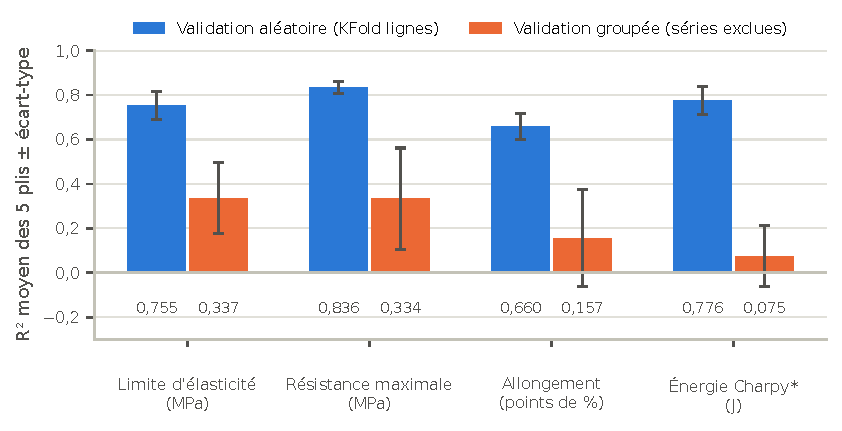
\includegraphics[width=\textwidth]{res_synthese_r2}
\caption{Résultat principal : $R^2$ moyen ($\pm$ écart-type sur 5 plis) de la
procédure supervisée avec sélection interne de la famille, configuration
16/médiane. Bleu : validation aléatoire ; orange : validation groupée.}
\label{fig:synthese}
\end{figure}

\begin{table}[htbp]
\centering
\small
\caption{Procédure supervisée avec sélection interne, configuration 16/médiane :
moyennes $\pm$ écart-type sur 5 plis externes, et MAE relative à la médiane de la cible.}
\label{tab:synthese}
\footnotesize
\setlength{\tabcolsep}{4pt}
\begin{tabular}{@{}l rrr rrr@{}}
\toprule
 & \multicolumn{3}{c}{Validation aléatoire} & \multicolumn{3}{c}{Validation groupée} \\
\cmidrule(lr){2-4}\cmidrule(lr){5-7}
Cible & MAE & MAE rel. & $R^2$ & MAE & MAE rel. & $R^2$ \\
\midrule
\YS{} (MPa)               & 31,630 $\pm$ 4,114 & 6,4\,\%  & 0,755 $\pm$ 0,063 & 56,757 $\pm$ 12,398 & 11,4\,\% & 0,337 $\pm$ 0,161 \\
\UTS{} (MPa)              & 23,861 $\pm$ 0,906 & 4,1\,\%  & 0,836 $\pm$ 0,027 & 54,344 $\pm$ 13,181 & 9,4\,\%  & 0,334 $\pm$ 0,228 \\
Allongement (pts de \%)   & 2,054 $\pm$ 0,239  & 7,7\,\%  & 0,660 $\pm$ 0,058 & 3,517 $\pm$ 0,516   & 13,2\,\% & 0,157 $\pm$ 0,220 \\
\charpy{} (J)             & 16,461 $\pm$ 1,161 & 16,5\,\% & 0,776 $\pm$ 0,062 & 35,752 $\pm$ 11,863 & 35,8\,\% & 0,075 $\pm$ 0,138 \\
\bottomrule
\end{tabular}
\end{table}

\paragraph{Lecture.} En validation aléatoire, l'erreur typique est de
\textbf{32\,MPa sur \YS{} et 24\,MPa sur \UTS}, soit 4 à 6\,\% de la valeur
médiane, et les $R^2$ dépassent 0,75 pour \YS, \UTS{} et Charpy. Par rapport à la
référence médiane, la MAE baisse de 55\,\% (\YS), 65\,\% (\UTS), 49\,\%
(allongement) et 55\,\% (Charpy). En validation groupée, les mêmes procédures
perdent une grande partie de leur pouvoir prédictif : la MAE ne baisse plus que
de 19\,\% (\YS), 25\,\% (\UTS), 14\,\% (allongement) et 1\,\% (Charpy) par rapport à
la référence. L'écart entre les deux scénarios est le résultat le plus
important du projet ; la \cref{sec:diag} en analyse les causes.

\subsection{Comparaison des familles de modèles}

Pour comprendre d'où viennent ces scores, chaque famille est aussi évaluée
séparément, avec ses hyperparamètres réglés en interne
(\cref{fig:familles}, \cref{tab:familles}).

\begin{figure}[htbp]
\centering
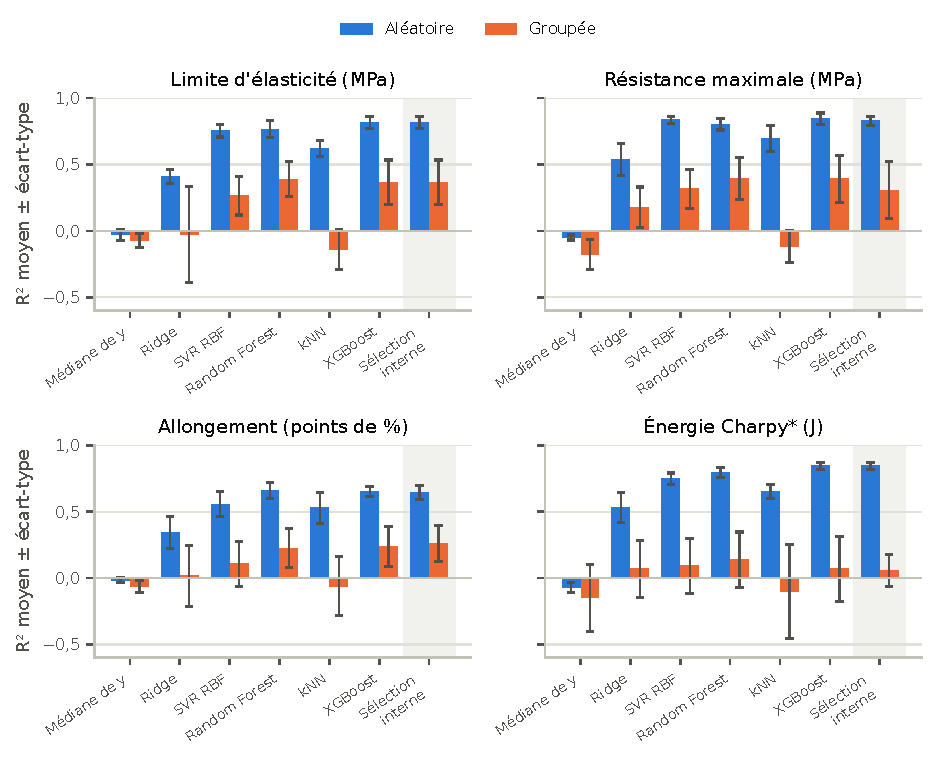
\includegraphics[width=\textwidth]{res_familles_r2}
\caption{$R^2$ moyen ($\pm$ écart-type) de chaque famille, configuration 16/médiane,
validations aléatoire et groupée. La dernière colonne (fond gris) est la procédure
de sélection interne de la famille.}
\label{fig:familles}
\end{figure}

\begin{table}[htbp]
\centering
\small
\caption{MAE moyenne et $R^2$ moyen par famille, configuration 16/médiane
(A : validation aléatoire ; G : validation groupée). En gras : meilleure famille par colonne.}
\label{tab:familles}
\setlength{\tabcolsep}{4pt}
\begin{tabular}{@{}l rr rr rr rr@{}}
\toprule
 & \multicolumn{2}{c}{\YS{} (MPa)} & \multicolumn{2}{c}{\UTS{} (MPa)} & \multicolumn{2}{c}{Allong. (pts)} & \multicolumn{2}{c}{\charpy{} (J)} \\
\cmidrule(lr){2-3}\cmidrule(lr){4-5}\cmidrule(lr){6-7}\cmidrule(lr){8-9}
Famille & A & G & A & G & A & G & A & G \\
\midrule
\multicolumn{9}{@{}l}{\emph{MAE}} \\
Médiane de $y$  & 70,03 & 70,45 & 68,88 & 72,66 & 4,02 & 4,09 & 36,76 & 36,04 \\
Ridge           & 54,05 & 69,39 & 44,32 & 61,90 & 3,01 & 3,66 & 26,91 & 34,75 \\
SVR RBF         & 31,75 & 59,35 & \meilleur{23,86} & 52,86 & 2,27 & 3,67 & 17,39 & 35,96 \\
Forêt aléatoire & \meilleur{31,24} & \meilleur{54,14} & 26,91 & \meilleur{48,91} & \meilleur{2,05} & \meilleur{3,34} & \meilleur{16,10} & \meilleur{33,03} \\
$k$NN           & 38,14 & 73,50 & 33,45 & 68,54 & 2,42 & 3,98 & 19,25 & 35,73 \\
\addlinespace
\multicolumn{9}{@{}l}{\emph{$R^2$}} \\
Médiane de $y$  & $-0{,}031$ & $-0{,}073$ & $-0{,}050$ & $-0{,}180$ & $-0{,}015$ & $-0{,}062$ & $-0{,}069$ & $-0{,}149$ \\
Ridge           & 0,412 & $-0{,}025$ & 0,538 & 0,179 & 0,345 & 0,016 & 0,529 & 0,069 \\
SVR RBF         & 0,754 & 0,264 & \meilleur{0,836} & 0,316 & 0,556 & 0,106 & 0,749 & 0,091 \\
Forêt aléatoire & \meilleur{0,765} & \meilleur{0,390} & 0,805 & \meilleur{0,394} & \meilleur{0,660} & \meilleur{0,226} & \meilleur{0,795} & \meilleur{0,138} \\
$k$NN           & 0,619 & $-0{,}140$ & 0,697 & $-0{,}115$ & 0,530 & $-0{,}060$ & 0,651 & $-0{,}099$ \\
\bottomrule
\end{tabular}
\end{table}

\paragraph{Analyse par famille.}
\begin{itemize}
  \item \textbf{Référence médiane.} Son $R^2$ est légèrement négatif, comme attendu : prédire la médiane du train est un peu moins bon que prédire la moyenne de la validation. Elle fixe le plancher.
  \item \textbf{Ridge.} Elle capte une partie du signal en aléatoire ($R^2$ de 0,35 à 0,54), mais presque rien en groupé. Une relation \emph{linéaire} globale ne suffit pas à décrire les propriétés.
  \item \textbf{SVR RBF et forêt aléatoire.} Ce sont les deux meilleures familles. La SVR est la meilleure pour \UTS{} en aléatoire ; la forêt est la meilleure partout ailleurs et la plus robuste en validation groupée. Les non-linéarités et interactions sont donc importantes.
  \item \textbf{$k$NN.} Très correct en aléatoire ($R^2$ de 0,53 à 0,70) mais \emph{négatif} en groupé. C'est un signal clair : une méthode purement locale prédit bien lorsqu'un voisin de la même série est présent dans le train, et échoue lorsque ce n'est plus le cas.
\end{itemize}

\begin{precaution}
La forêt aléatoire isolée peut afficher un meilleur score externe que la
procédure de sélection interne (par exemple 0,390 contre 0,337 pour \YS{} en
groupé). Choisir la forêt \emph{après} avoir lu ce tableau reviendrait à
sélectionner sur la validation : seul le score de la sélection interne est une
estimation honnête de la procédure complète.
\end{precaution}

\subsection{Familles et hyperparamètres sélectionnés}

La sélection interne peut choisir une famille différente selon le pli. Les
\cref{tab:selection_aleatoire,tab:selection_groupee} détaillent ces choix.

\begin{table}[htbp]
\centering
\small
\caption{Validation aléatoire : famille et hyperparamètres choisis par la MAE
interne dans chaque pli externe, et scores externes obtenus.}
\label{tab:selection_aleatoire}
\setlength{\tabcolsep}{4pt}
\begin{tabular}{@{}l c l l r r@{}}
\toprule
Cible & Pli & Famille & Hyperparamètres & MAE & $R^2$ \\
\midrule
\YS     & 0 & SVR RBF & $C=10$, $\varepsilon=0{,}05$, $\gamma=0{,}05$ & 28,27 & 0,769 \\
        & 1 & Forêt   & feuille 1, prof. libre, \texttt{mf} 0,5 & 29,26 & 0,817 \\
        & 2 & Forêt   & feuille 1, prof. libre, \texttt{mf} 0,5 & 35,67 & 0,671 \\
        & 3 & SVR RBF & $C=10$, $\varepsilon=0{,}05$, $\gamma$=scale & 28,42 & 0,807 \\
        & 4 & SVR RBF & $C=10$, $\varepsilon=0{,}05$, $\gamma$=scale & 36,54 & 0,710 \\
\midrule
\UTS    & 0--4 & SVR RBF & $C=10$, $\varepsilon=0{,}05$, $\gamma \in \{0{,}05;\text{scale}\}$ & 23,1--25,4 & 0,814--0,871 \\
\midrule
Allong. & 0--4 & Forêt & feuille 1, prof. libre, \texttt{mf} $\in\{0{,}5; 1\}$ & 1,84--2,42 & 0,569--0,728 \\
\midrule
Charpy  & 0, 1, 3, 4 & Forêt & feuille 1, prof. libre, \texttt{mf} $\in\{0{,}5; 1\}$ & 14,9--17,5 & 0,756--0,849 \\
        & 2 & SVR RBF & $C=100$, $\varepsilon=0{,}05$, $\gamma=0{,}05$ & 17,51 & 0,683 \\
\bottomrule
\end{tabular}
\end{table}

\begin{table}[htbp]
\centering
\small
\caption{Validation groupée : famille et hyperparamètres choisis par la MAE
interne dans chaque pli externe, et scores externes obtenus.}
\label{tab:selection_groupee}
\setlength{\tabcolsep}{4pt}
\begin{tabular}{@{}l c l l r r@{}}
\toprule
Cible & Pli & Famille & Hyperparamètres & MAE & $R^2$ \\
\midrule
\YS     & 0 & Forêt   & feuille 2, prof. libre, \texttt{mf} 0,5 & 43,62 & 0,472 \\
        & 1 & Forêt   & feuille 1, prof. libre, \texttt{mf} 0,5 & 68,48 & 0,204 \\
        & 2 & SVR RBF & $C=10$, $\varepsilon=0{,}05$, $\gamma=0{,}05$ & 49,94 & 0,273 \\
        & 3 & Forêt   & feuille 1, prof. 10, \texttt{mf} 0,5 & 50,28 & 0,543 \\
        & 4 & SVR RBF & $C=10$, $\varepsilon=0{,}2$, $\gamma=0{,}05$ & 71,46 & 0,191 \\
\midrule
\UTS    & 0 & Ridge   & $\alpha=100$ & 74,90 & 0,038 \\
        & 1 & Forêt   & feuille 1, prof. libre, \texttt{mf} 0,5 & 49,49 & 0,155 \\
        & 2 & SVR RBF & $C=10$, $\varepsilon=0{,}05$, $\gamma=0{,}05$ & 38,76 & 0,399 \\
        & 3 & Forêt   & feuille 2, prof. 10, \texttt{mf} 0,5 & 52,60 & 0,555 \\
        & 4 & Forêt   & feuille 2, prof. libre, \texttt{mf} 0,5 & 55,98 & 0,523 \\
\midrule
Allong. & 0, 1, 3 & Forêt & \texttt{mf} 0,5, feuille 5/2/5 & 2,86--3,63 & 0,166--0,468 \\
        & 2, 4 & SVR RBF & $\varepsilon=0{,}2$, $\gamma=0{,}05$, $C=1$/$10$ & 3,61--4,25 & $-0{,}080$--$-0{,}022$ \\
\midrule
Charpy  & 0, 1 & SVR RBF & $C=1$, $\varepsilon=0{,}2$, $\gamma=0{,}05$ & 31,00 / 27,33 & $-0{,}038$ / 0,222 \\
        & 2, 4 & Médiane de $y$ & -- & 24,24 / 44,12 & $-0{,}034$ / $-0{,}006$ \\
        & 3 & Forêt   & feuille 1, prof. libre, \texttt{mf} 1 & 52,09 & 0,228 \\
\bottomrule
\end{tabular}
\end{table}

Plusieurs enseignements ressortent. En aléatoire, les choix sont
\textbf{stables} : SVR ($C=10$, $\varepsilon=0{,}05$) pour \UTS{} dans les cinq
plis, forêt à feuilles de taille 1 pour l'allongement. Les modèles peu
régularisés sont préférés, ce qui est cohérent avec un contexte où des voisins
très proches existent dans le train. En groupé, les choix sont \textbf{instables}
--- Ridge, SVR ou forêt pour \UTS{} selon le pli --- et la boucle interne
retient même la \textbf{référence médiane} dans deux plis Charpy : en l'absence
de séries connues, aucun modèle ne bat de façon fiable la constante pour cette
cible. Cette instabilité illustre l'incertitude du transfert entre séries.

\subsection{Prédictions et observations}

La \cref{fig:obs_pred} compare les prédictions hors pli aux valeurs observées.

\begin{figure}[htbp]
\centering
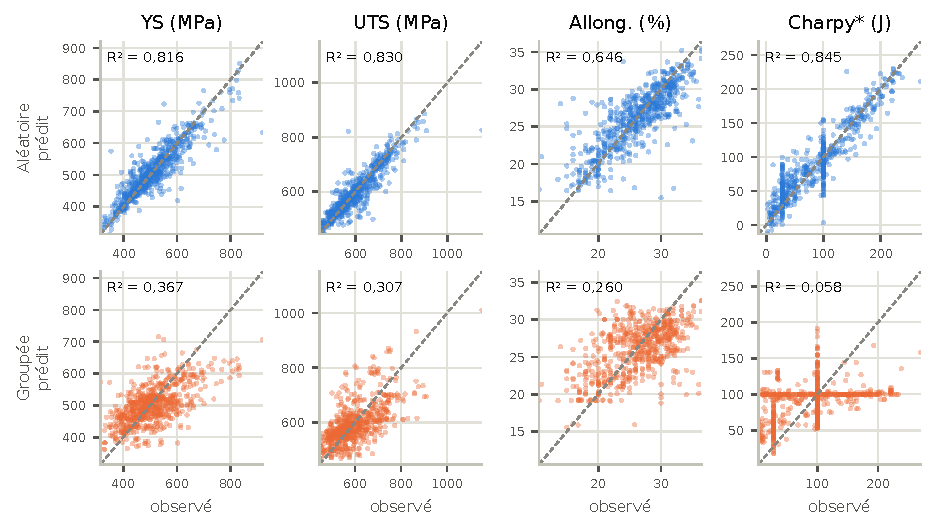
\includegraphics[width=\textwidth]{res_observe_predit}
\caption{Valeurs observées et prédites hors pli (OOF) par la procédure de
sélection interne, configuration 16/médiane. Haut : validation aléatoire ; bas :
validation groupée. La diagonale pointillée correspond à une prédiction parfaite.}
\label{fig:obs_pred}
\end{figure}

En validation aléatoire, les points suivent la diagonale. En validation groupée,
le nuage est \textbf{aplati} : les prédictions restent proches de la moyenne et
les fortes valeurs de \YS{} et \UTS{} sont sous-estimées. Pour Charpy, on
distingue des bandes verticales à 28 et 100\,J : pour ces couples, le modèle
prédit des énergies très variées alors que l'énergie observée est fixée par le
protocole, ce qui est cohérent avec l'hypothèse de températures de transition.

\subsection{Modèles réentraînés pour l'inférence}

Une fois l'évaluation terminée, chaque famille est réglée par une nouvelle CV5
sur \emph{tous} les labels (aléatoire, graine 1042, ou par groupes), puis
réentraînée. La famille de plus faible MAE de sélection est retenue par cible
(\cref{tab:modeles_finaux}). Ces MAE de sélection sont optimistes et \textbf{ne
remplacent pas} les scores imbriqués ; ces modèles ont vu tous les labels et ne
servent jamais à scorer les plis.

\begin{table}[htbp]
\centering
\small
\caption{Modèles supervisés réentraînés sur tous les labels, retenus pour l'inférence.}
\label{tab:modeles_finaux}
\begin{tabular}{@{}l l l r l@{}}
\toprule
CV de choix & Cible & Famille & MAE de sélection & Hyperparamètres \\
\midrule
Aléatoire & \YS     & SVR RBF & 31,228 & $C=10$, $\varepsilon=0{,}05$, $\gamma$=scale \\
          & \UTS    & SVR RBF & 24,060 & $C=10$, $\varepsilon=0{,}05$, $\gamma=0{,}05$ \\
          & Allong. & Forêt   & 1,940  & feuille 1, prof. libre, \texttt{mf} 0,5 \\
          & Charpy  & Forêt   & 15,387 & feuille 1, prof. libre, \texttt{mf} 1 \\
\midrule
Groupée   & \YS     & Forêt   & 58,695 & feuille 2, prof. libre, \texttt{mf} 0,5 \\
          & \UTS    & SVR RBF & 46,555 & $C=10$, $\varepsilon=0{,}05$, $\gamma=0{,}05$ \\
          & Allong. & Forêt   & 3,282  & feuille 1, prof. libre, \texttt{mf} 0,5 \\
          & Charpy  & Forêt   & 32,375 & feuille 1, prof. 10, \texttt{mf} 0,5 \\
\bottomrule
\end{tabular}
\end{table}

Au total, \textbf{80 pipelines supervisées} sont exportées (40 par protocole :
20 modèles de plis externes et 20 réapprentissages complets), avec leur
prétraitement, leurs métadonnées (entrées, unités, identifiants du train,
paramètres, versions) et leur empreinte SHA-256. Toutes ont été rechargées dans
un processus Python neuf et les modèles de plis reproduisent exactement leurs
prédictions hors pli.

\begin{aretenir}
\begin{itemize}[leftmargin=1.2em]
  \item Configuration initiale 13/itérative : gains modestes, $R^2 \leq 0{,}19$ en validation groupée.
  \item Configuration 16/médiane : $R^2$ de \textbf{0,66 à 0,84 en aléatoire}, mais \textbf{0,08 à 0,34 en groupé}.
  \item \textbf{Forêt aléatoire et SVR RBF} sont les meilleures familles ; le $k$NN s'effondre dès que la série est absente.
  \item Les choix internes sont stables en aléatoire, instables en groupé.
\end{itemize}
\end{aretenir}
